\secnumbersection{MARCO CONCEPTUAL}

Para abordar nuestro problema, primero debemos definir algunos conceptos que han
sido mencionados en las secciones anteriores de forma más formal, tales como, la
\textit{web} semántica, \textit{SPARQL}, \textit{RDF} y el contexto en el que
estos se utilizan. Para esto, nos apoyaremos en las siguientes definiciones.

\subsection{\textit{Web} Semántica}

La red informática mundial, \textit{World Wide Web} o simplemente \textit{Web}
es el sistema de información público más importante desarrollado en los últimos
30 años, el cual permite la transmisión de documentos electrónicos identificados
por URIs \textit{(Uniform Resource Identifiers)}, los cuales pueden estar
enlazados a otros documentos a través de hipertexto y que se encuentran
disponibles utilizando servicios de la internet.

La \textit{World Wide Web} fue diseñada como un espacio para la información con
el objetivo de no solo ser útil para las comunicaciones entre humanos, sino que
también un lugar donde las máquinas podrían ayudar y participar. Sin embargo,
uno de los principales problemas de la \textit{Web} es que la mayor parte de su
contenido ha sido diseñado para ser consumido por humanos, lo que implica que
para las máquinas y el software no es fácil acceder e interpretar el contenido
disponible, incluso si este proviene de una base de datos estructurada a través
de columnas claras y tipificadas. La \textit{web} semántica busca desarrollar
herramientas, lenguajes, protocolos y estándares que permitan, tanto a maquinas
como humanos, procesar toda la información disponible en la \textit{Web}. En
base a esto, podemos definir a la \textit{web} semántica como la idea de generar
una red de datos en la \textit{Web}, hasta cierto punto, una base de datos
global.
\cite{berners1998semantic}

\subsection{Arquitectura de la \textit{web} semántica}

La \textit{web} semántica está construida en base a múltiples bloques, los
cuales representan estándares y lenguajes utilizados para lograr determinadas
funcionalidades descritas en su arquitectura \cite{harth2011semantic}, una
representación gráfica de esta arquitectura en bloques se puede observar en la
figura \ref{fig:semantic-web-arq}, la cual, podemos describir en las siguientes
capas.

\begin{figure}
    \centering
    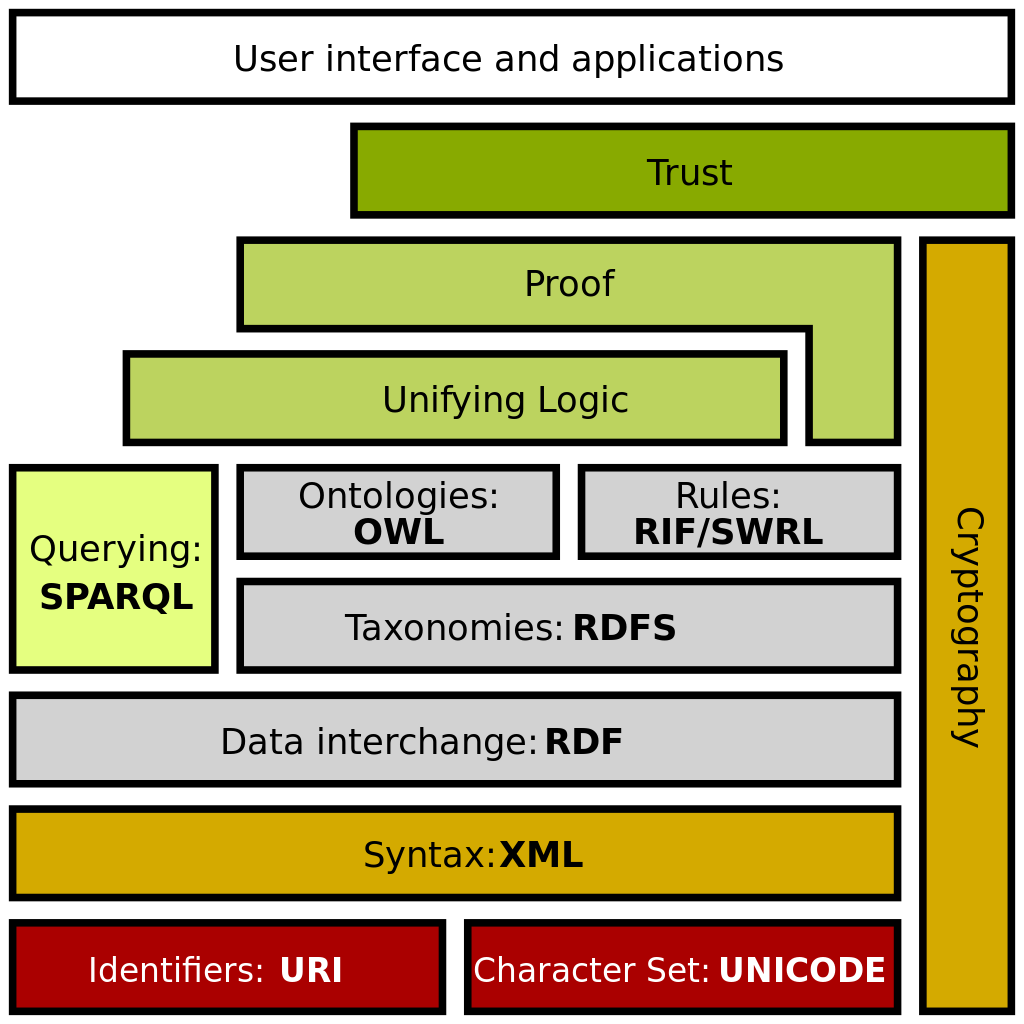
\includegraphics[width=0.6\linewidth]{semantic_web_stack}
    \caption{Arquitectura de la \textit{web} semántica.} Fuente:
    \textit{Semantic Web Stack}. Wikipedia.
    \label{fig:semantic-web-arq}
\end{figure}

\subsubsection{Referencias, transporte y principios de los datos enlazados}
\label{sec:refs-transporte-enlazados}

El acceso a los datos es fundamental para la arquitectura de la \textit{web}
semántica. Podemos tomar como referencia, el modelo utilizado por los servidores
\textit{Web}, en el cual, los documentos disponibles se encuentran enlazados a
otros de forma descentralizada, esto es, que el documento referenciado no
necesariamente se encuentra en el mismo servidor que está haciendo referencia a
él. Estos enlaces, son utilizados por los usuarios para navegar entre los
millones de servidores disponibles en la \textit{Web}.

Las URI/IRI y el protocolo HTTP son parte fundamental del núcleo que define
tanto a la \textit{World Wide Web} como a la \textit{web} semántica. En un
ejemplo concreto, la URI \url{https://en.wikipedia.org/wiki/Back_to_the_Future}
en la \textit{Web}, representa el documento en el servidor
\url{https://www.wikipedia.org} que contiene información sobre la serie de
películas y obras de título ``Volver al Futuro'', en cambio, en el contexto de
la \textit{web} semántica, la URI \url{https://www.wikidata.org/wiki/Q1}
representa al ``universo'' como una entidad, la cual es parte del
\url{https://www.wikidata.org/wiki/Q3327819} ``multiverso'' y es estudiado por
la \url{https://www.wikidata.org/wiki/Q338} ``cosmología''.

Los datos del ejemplo anterior son publicados por ``The Wikipedia Fundation" a
través del servicio Wikidata \cite{vrandevcic2014wikidata}, pero las relaciones
descritas podrían enlazar a otros editores de contenido, como por ejemplo
DBpedia \cite{valsecchi2015dbpedia}, el cual es un esfuerzo comunitario para
extraer información estructurada desde distintas fuentes y enlazarlas a través
del formato \textit{RDF}. Para lograr esto, los editores de contenido para la
\textit{web} semántica aplican los siguientes principios a sus datos, los cuales
son conocidos como los ``principios para datos enlazados'' o \textit{LinkedData
principles} \cite{bizer2011linked}.

\begin{enumerate}
    \item Utilizar URIs como nombres para entidades.
    \item Utilizar URIs HTTP para que los usuarios puedan buscar y acceder a
    estas entidades.
    \item Cuando un usuario consulta una URI, debes entregar información
    relevante, utilizando estándares como \textit{RDF} y \textit{SPARQL}.
    \item Debes incluir enlaces a otras URIs, para que los usuarios descubran
    más entidades.
\end{enumerate}

\subsubsection{Intercambio de datos}
\label{sec:intercambio-datos}

\begin{figure}
    \centering
    \includesvg[width=\linewidth]{rdf-graph.svg}
    \caption{Un grafo \textit{RDF} básico.} Los nodos \textit{Subject} y
    \textit{Object} están conectados a través de la relación \textit{Predicate}.
    Fuente: \textit{RDF 1.1 Concepts and Abstract Syntax. World Wide Web
    Consortium}.
    \label{fig:rdf-graph1}
\end{figure}

Los datos de la \textit{web} semántica son generados por distintas entidades al
rededor del mundo, las cuales no están necesariamente coordinados entre ellos,
por lo que la arquitectura debe soportar la creación distribuida de datos junto
con la integración de múltiples fuentes y la interoperabilidad entre los datos
creados \cite{bizer2011linked}. Este tipo de requerimientos los cumplen las
estructuras de datos basados en grafos como \textit{RDF}. \textit{RDF} es un
formato basado en la descripción de grafos dirigidos, los cuales representan la
información de la forma de tríos sujeto - predicado - objeto, en la cual, el
sujeto y el predicado corresponden a nodos del grafo y el predicado es un arco
que los relaciona como se puede observar en la figura \ref{fig:rdf-graph1}. En
estos tríos, cualquiera de estos objetos puede tomar el valor de una URI, un
valor literal (cadenas de texto, números o fechas) o simplemente un nodo vacío
(identificadores que no pueden ser referenciados por otra entidad).

\textit{RDF} corresponde a la especificación de un lenguaje abstracto para
describir relaciones entre entidades, el cual, puede ser serializado en
múltiples formatos de texto como \textit{Extensible Markup Language (XML)}
\cite{beckett2004rdf} en la figura \ref{fig:rdf-xml-ex} o en un formato más
compacto como \textit{Turtle} \cite{beckett2014rdf} en la figura
\ref{fig:rdf-turtle-ex}.

\begin{figure}
    \centering
    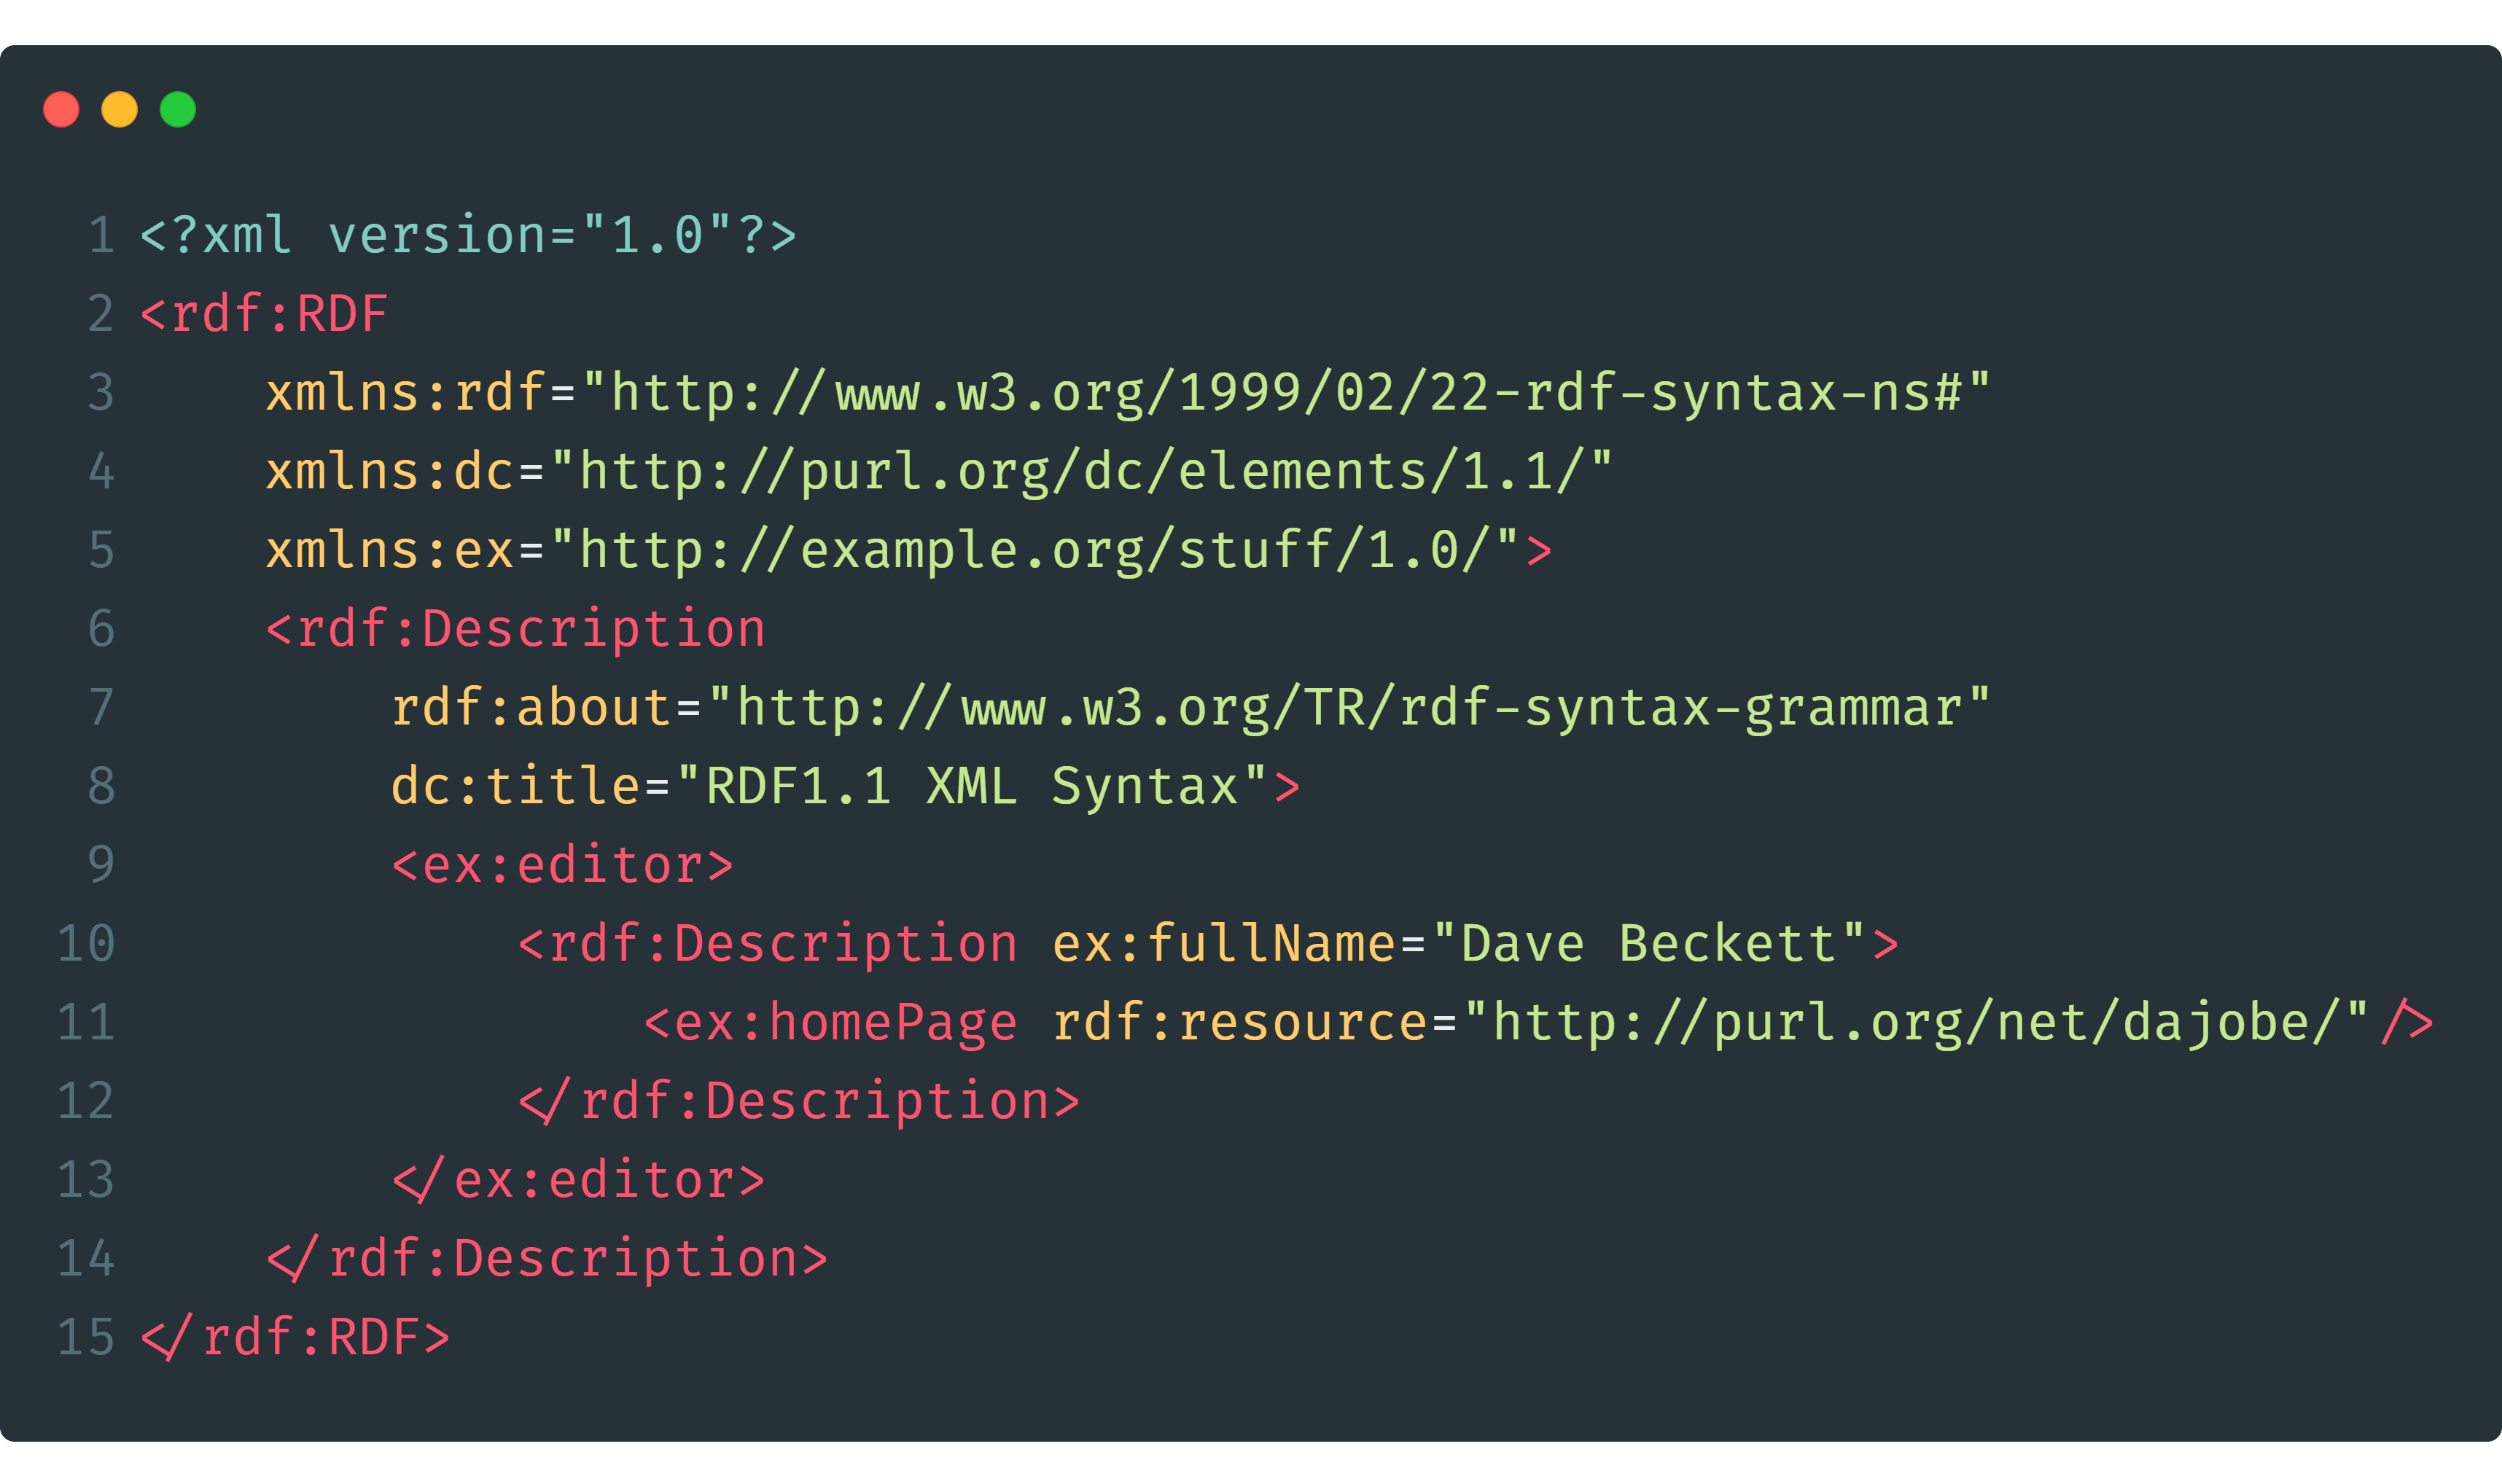
\includegraphics[width=\linewidth]{rdf-xml-ex.png}
    \caption{Descripción de un documento \textit{RDF/XML}.} Fuente: RDF 1.1 XML
    Syntax. World Wide Web Consortium.
    \label{fig:rdf-xml-ex}
\end{figure}

\begin{figure}
    \centering
    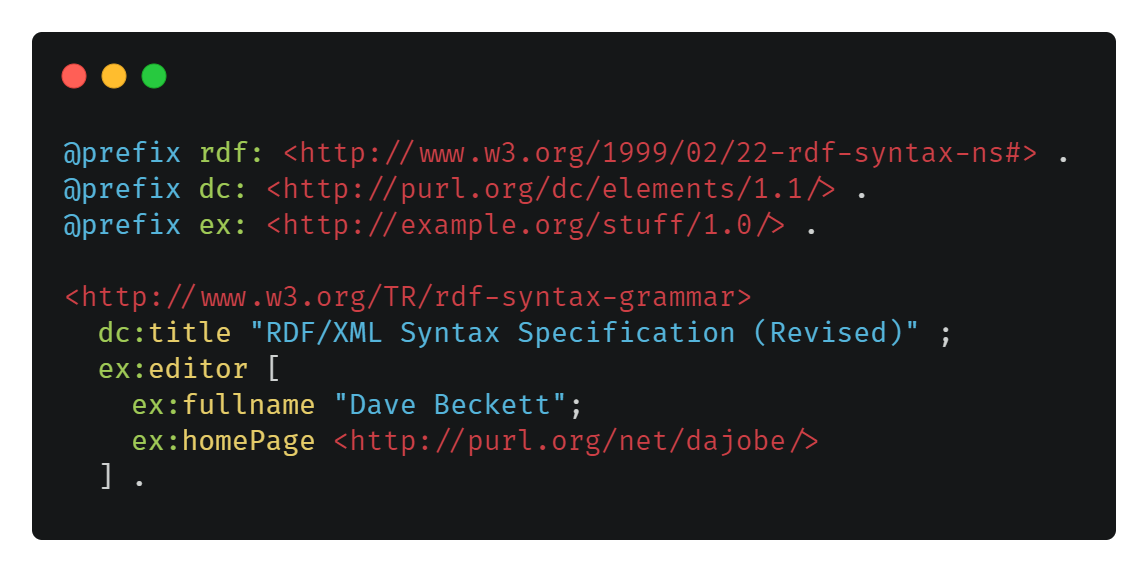
\includegraphics[width=\linewidth]{rdf-turtle-ex.png}
    \caption{Descripción de un documento \textit{RDF/Turtle}.} Fuente: Turtle
    (Syntax). Wikipedia.
    \label{fig:rdf-turtle-ex}
\end{figure}

\subsubsection{Consultas y actualizaciones}

Los principios de los datos enlazados explicados en la sección
\ref{sec:intercambio-datos} nos entregan guias sobre como realizar la
publicación y permitir el acceso a datos simples, sin embargo, no es posible
realizar consultas complejas a aquellos datos publicados utilizando estos
principios, puesto que, no es necesario contar con un sistema o mecanismo de
consulta para publicar información. Si continuamos con el ejemplo de las
peliculas ``Volver al Futuro'', consideremos que buscamos obtener los titulos de
aquellas peliculas en las que los miembros del elenco de ``Volver al Futuro''
también han actuado. Una forma relativamente sencilla de lograr esto, es acceder
a la URI que representa la pelicula, obtener las URIs de los actores y de forma
iterativa acceder a estas URIs para obtener el nombre de las peliculas en las
que cada miembro ha participado. No es dificil darse cuenta, que este proceso no
es para nada eficiente en tiempo de ejecución ni recursos de red utilizados.

Para resolver esta consulta, utilizamos el lenguaje de consultas para
repositorios \textit{RDF} llamado \textit{SPARQL}, cuyo nombre corresponde al
acronimo recursivo ``\textit{\textbf{S}PARQL \textbf{P}rotocol \textbf{A}nd
\textbf{R}DF \textbf{Q}uery \textbf{L}anguage}'' \cite{world2013sparql}. Este
lenguaje esta diseñado para evaluar consultas hacia repositorios de datos
almacenados en formato \textit{RDF}, en estos repositorios, la información no se
obtiene accediendo de forma iterativa a distintas URIs que representan
entidades, si no que enviando consultas a un
\textit{endpoint}\footnote{\textit{Endpoint:} Del inglés punto final. Se refiere
a un punto en la red expuesto por un sistema informático con el cual se puede
interactuar o establecer un canal de comunicaciones.} que soporta
\textit{SPARQL}. \textit{SPARQL} permite a sus usuarios especificar URIs
arbitrarias, las cuales podrian no ser accesibles a través de la \textit{Web},
junto con un patron de grafo dirigido el cual debe coincidir con los datos
disponibles en el repositorio y en el que pueden ser descritas determinadas
restricciones para los datos obtenidos. En la figura \ref{fig:graph-pattern-ex}
se puede apreciar el patron del grafo utilizado para consultar por las peliculas
en las que el elenco de ``Volver al futuro'' ha participado.

\begin{figure}
    \centering
    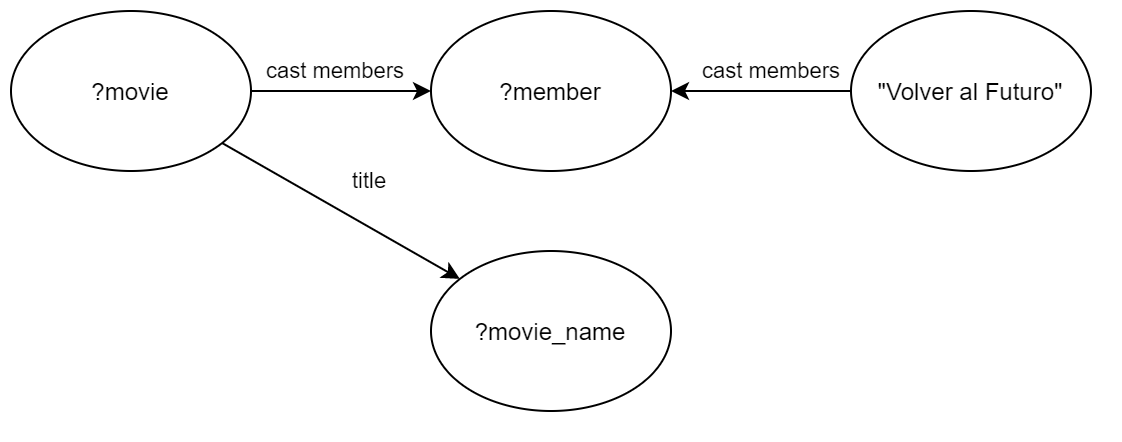
\includegraphics[width=\linewidth]{graph-pattern-ex.png}
    \caption{Patrón de un grafo \textit{RDF} básico. } Fuente: Elaboración
    propia.
    \label{fig:graph-pattern-ex}
\end{figure}

Esta consulta puede ser representada utilizando \textit{SPARQL}, como se puede
apreciar en la figura \ref{fig:graph-pattern-ex-sparql}. Una consulta
\textit{SPARQL} esta compuesta de multiples secciones, las sentencias
\textit{\texttt{PREFIX}} son utilizadas para abreviar URIs y su rol es apoyar la
legibilidad de la consulta. El nucleo de una consulta se encuentra en la sección
\textit{\texttt{WHERE}}, en la cual, se debe definir de forma precisa el patrón
de nuestro grafo dirigido, el cual debe coincidir con la información semántica
disponible. Un patrón básico consiste de patrones individuales los cuales pueden
ser sujetos, predicados u objetos unidos por variables, formando una plantilla,
la cual será completada en el proceso de evaluación de la consulta. De forma
opcional, una sentencia \textit{\texttt{WHERE}} puede estar acompañada de una
expresión \textit{\texttt{FILTER}} la cual puede acotar los resultados obtenidos
a determinadas estrucutras que cumplan con creiterios especificados.

\begin{figure}
    \centering
    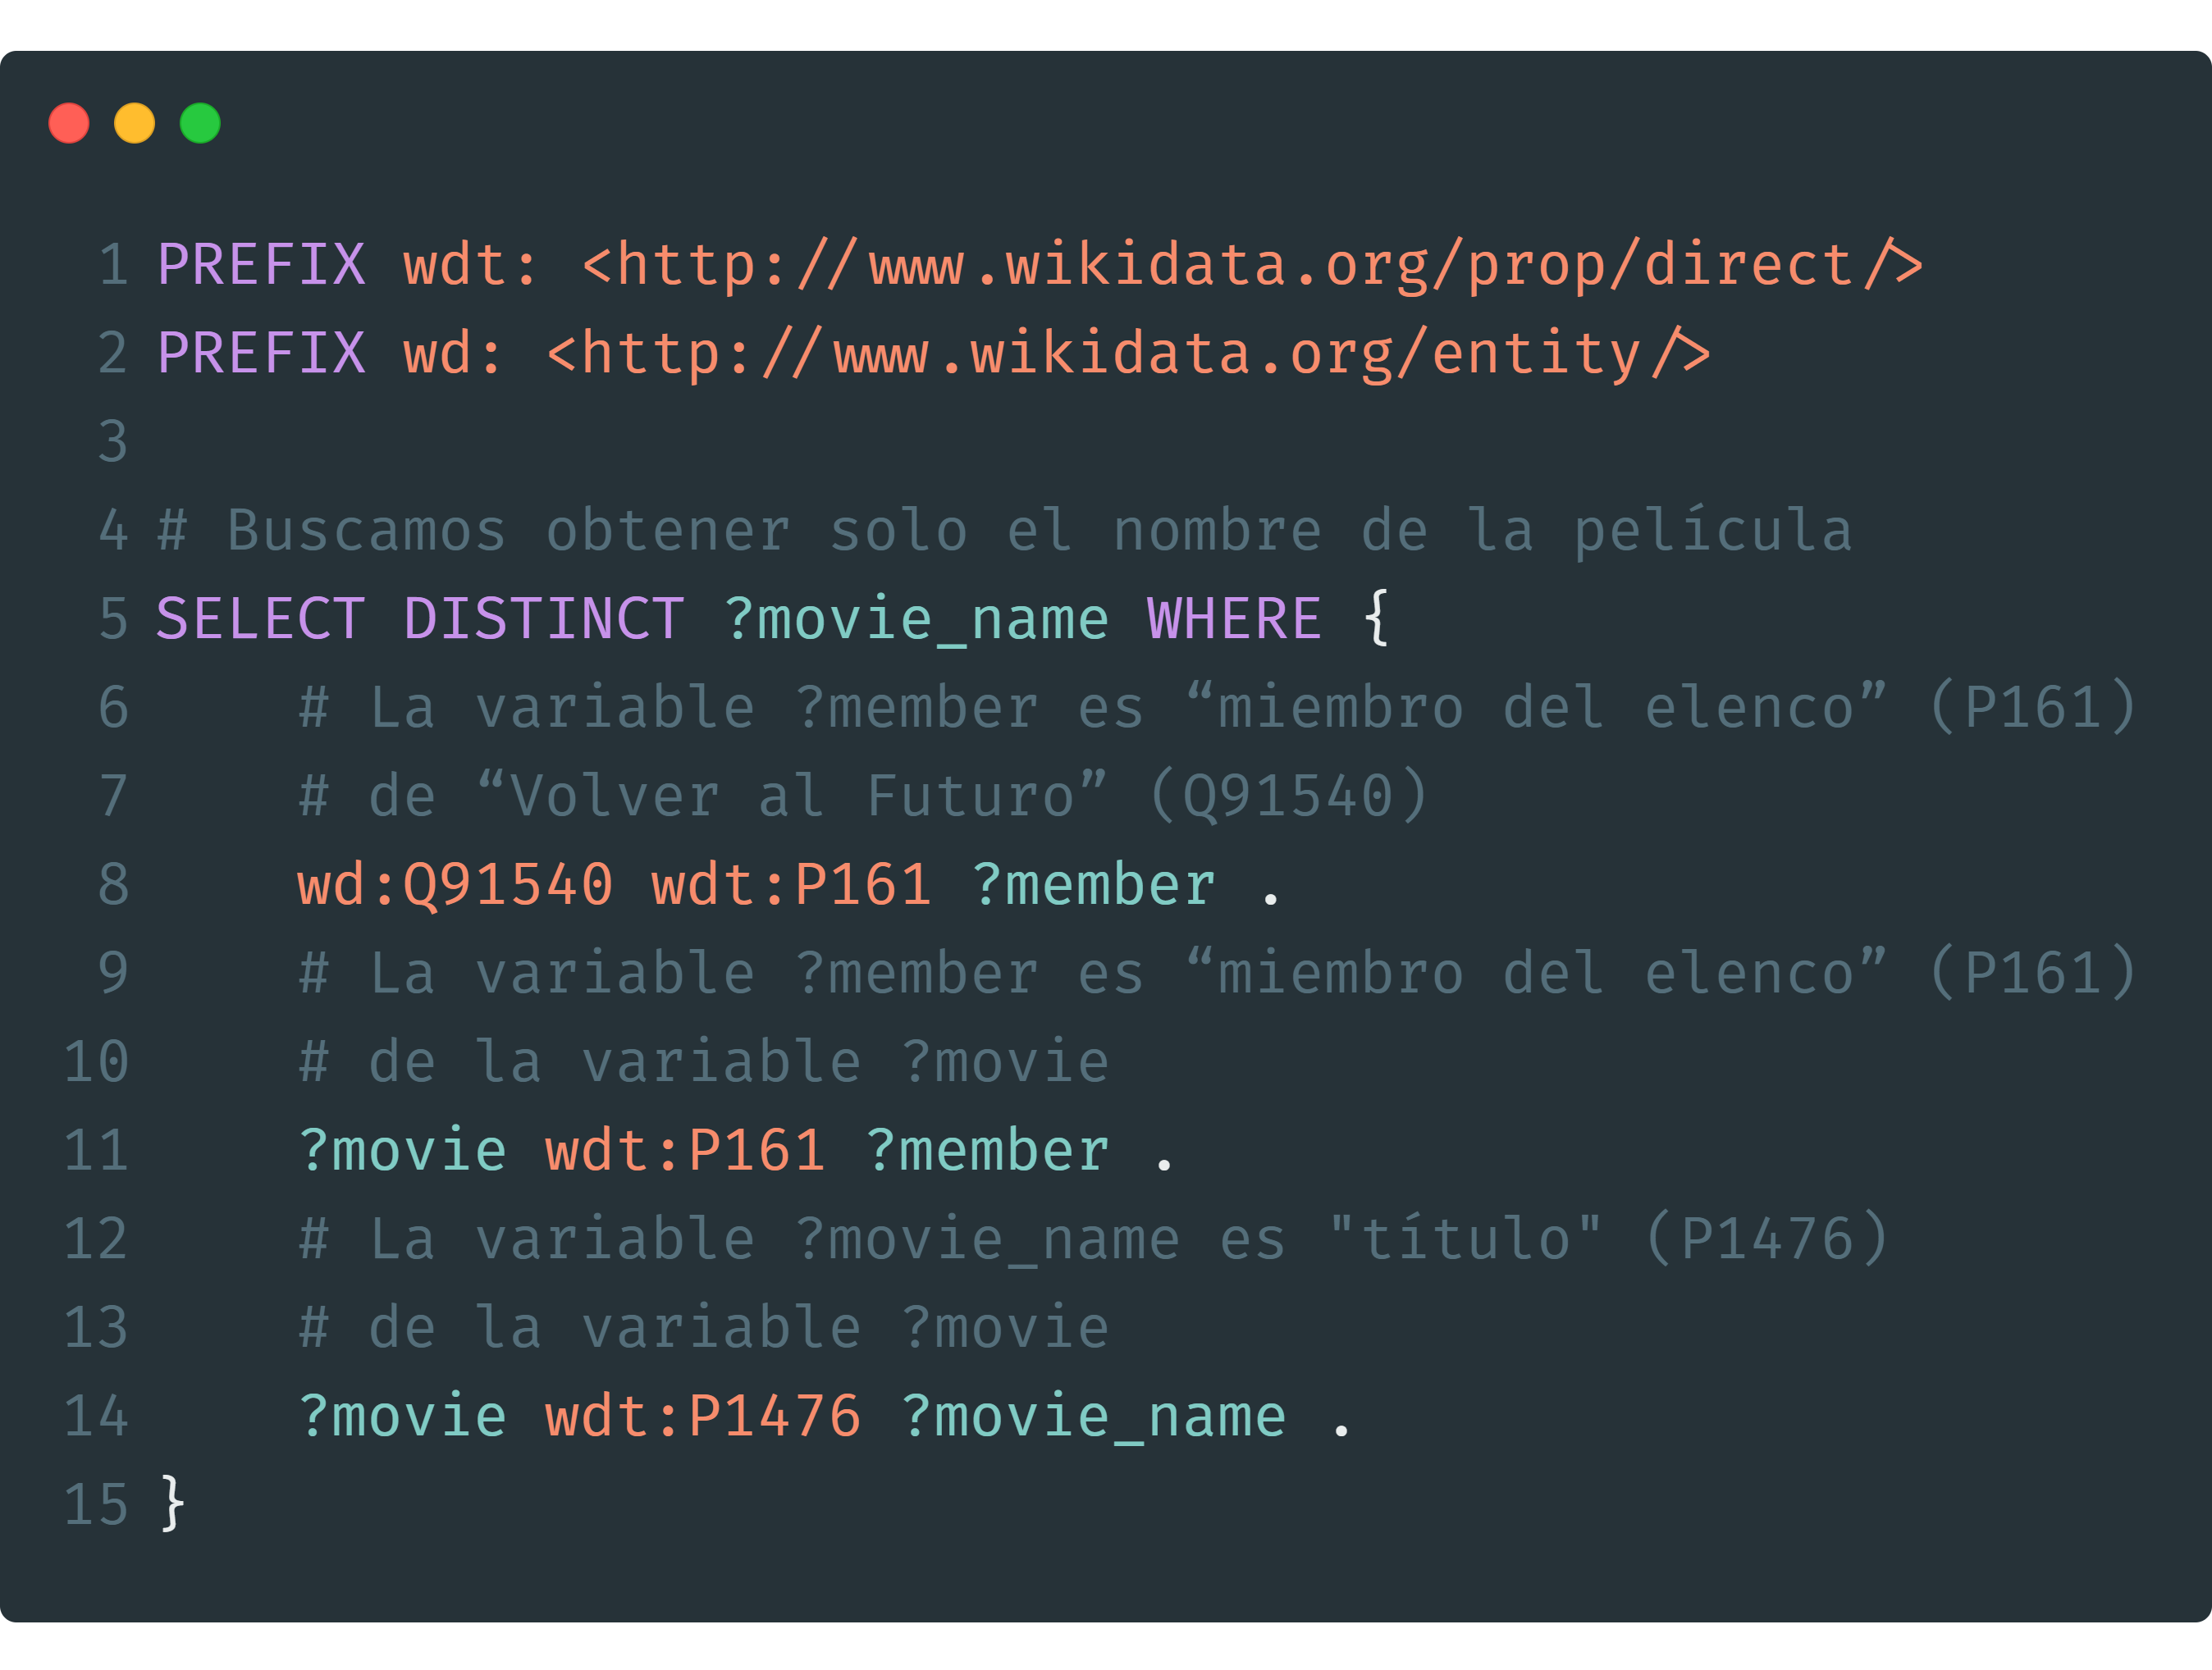
\includegraphics[width=0.85\linewidth]{graph-pattern-ex-sparql.png}
    \caption{Una consulta \textit{SPARQL} realizada al servicio Wikidata.}
    Fuente: Elaboración propia.
    \label{fig:graph-pattern-ex-sparql}
\end{figure}

% FIXME: Updated ranking of implementations

La especificación \textit{SPARQL} puede ser implementada en multiples
repositorios orientados a grafos, entre los populares se encuentran Sesame
\cite{broekstra2002sesame}, Jena \cite{mcbride2001jena}, Virtuoso
\cite{openlink2015virtuoso}, BigData \cite{thompson2016bigdata}, OWLIM
\cite{kiryakov2005owlim} y RDF-3X \cite{neumann2010rdf}. Debido a que en muchas
ocaciones los datos estan almacenados en bases de datos relacionales, se
necesitan \textit{wrappers}\footnote{\textit{Wrapper:} Del inglés envoltorio.
Una función o segmento de \textit{software} que ejecuta a otras funciones ya sea
por comodidad o para mejorar la compatibilidad o interoperabilidad del
\textit{software} ejecutado.} que nos permitan acceder a estos datos a través de
\textit{APIs}. Ejemplos conocidos de estos \textit{wrappers} son D2R
\cite{bizer2006d2r} y Triplify \cite{auer2009triplify}. Estas herramientas
permiten que fuentes de datos legadas puedan ser expuestas y consultadas como
grafos semánticos, lo cual facilita la transición hacia estas nuevas
técnologias.

Además de la especificación de un lenguaje, \textit{SPARQL} define los
protocolos de acceso y formatos interoperables para los conjuntos de datos
almacenados. Los datos son expuestos a través de HTTP lo cual permite un libre
acceso y elimina la necesidad de los usuarios de descargar estos datos para
consultarlos.

Actualmente el estándar \textit{SPARQL} permite realizar consultas a una unica
fuente de datos a la vez. Para acceder a datos de multiples fuentes al mismo
tiempo es posible realizar multiples consultas secuenciales a los distintos
repositorios, sin embargo, la responsabilidad de unir estos resultados de forma
consistente pasa a ser del usuario que realiza la consulta. Actualmente se esta
diseñando una solución alternativa para realizar consultas federadas. [FIXME:
ESTO PARECE DESACTUALIZADO, BUSCAR UNA MEJOR FUENTE]

\subsubsection{Ontologías y razonamiento}
\label{sec:ontologia-y-razonamiento}

Para codificar un significado a nuestros datos debemos utilizar construcciones
logicas. Las técnologias que habilitan el razonamiento para la \textit{web}
semántica son los esquemas \textit{RDF}, el lenguaje de
ontologías\footnote{Ontología: En el campo de la informática, corresponde a una
definición formal de tipos, propiedades y relaciones entre distintas entidades
las cuales pertenecen a un determinado conjunto o dominio.} \textit{OWL (Web
Ontology Language)} \cite{antoniou2004web} y \textit{RIF (Rule Interchange
Format)} \cite{kifer2008rule}.

Para explicar el razonamiento en la \textit{web} semántica, esto es, generar
conclusiones en base a hechos y verdades disponibles en nuestros repositorios de
datos, podemos utilizar un conjunto de ontologías aplicado al ejemplo que hemos
utilizado en las secciones anteriores a través de las propiedades
\texttt{rdfs:subClassOf} y \texttt{owl:sameAs}. La propiedad
\texttt{rdfs:subClassOf} puede ser utilizada para definir jerarquias de clases.
Consideremos el siguiente ejemplo, definiremos una ontología llamada
\texttt{OntologíaFormula1} en el contexto de la competencia de automovilismo
internacional, esta ontología define dos clases: \texttt{f1:Competidores},
\texttt{f1:Equipo} y contiene un axioma\footnote{Axioma: Una sentencia que debe
ser considerada verdadera y que se utiliza como primisa para realizar futuros
rezonamientos o argumentos.} el cual indica que \texttt{f1:Equipo} es una
subclase de \texttt{f1:Competidores} a través de la propiedad
\texttt{rdfs:subClassOf}. Esta relación le permite a un agente inteligente
deducir que las instancias de \texttt{f1:Equipo} también son del tipo
\texttt{f1:Competidores}, de esta forma si en nuetro repositorio existen los
registros ``Charles Leclerc'' del tipo \texttt{f1:Competidores} y ``Ferrari''
del tipo \texttt{f1:Equipo}, cuando realizemos una consulta por todas las
entidades del tipo \texttt{f1:Competidores} obtendremos como resultado ``Charles
Leclerc'' y ``Ferrari'' incluso cuando las instancias no especifican esta
relación de forma explicita.

Otra propiedades importante es \texttt{owl:sameAs}, la cual puede ser usada para
especificar que dos recursos son identicos, incluso cuando se encuentran en
repositorios distintos. Por ejemplo, podemos indicar que el recurso
\url{https://www.wikidata.org/wiki/Q27586} es identico a
\url{http://dbpedia.org/page/Ferrari}, lo que permite a nuestro agente
inteligente consolidar información más completa para una entidad determinada
desde multiples fuentes de datos.

\subsubsection{Reglas}

Otro mecanismo que nos permite generar conclusiones en base a datos existentes
son las regals logicas. Estas reglas estan compuestas de dos secciones,
antecedentes y consequencias: si se cumplen las sentencias en los antecedentes,
entonces las sentencias en las consequencias son verdaderas. La \textit{W3C}
recomienda utilizar \textit{RIF} \cite{kifer2013rif} para intercambiar reglas
entre sistemas. El conjunto común de reglas utilizadas en multiples sistemas ha
sido estandarizado en \textit{RIF Core} \cite{boley2010rif}.

\subsubsection{Seguridad y encriptación}

En un sistema global abierto como la \textit{Internet}, donde la información es
transmitida a través de canales inseguros y sin autenticación utilizando
infraestrucutura mantenida por una gran cantidad de organizaciones es necesario
definir mecanismos y protocolos para realizar intercambios de información de
forma segura. Estos problemas son abordados utilizando la capa de criptografia
en la \textit{web} semántica.

Para asegurar que los datos no son alterados durante su transmisión se utiliza
el protocolo HTTPS \cite{rescorla2000rfc2818} el cual implementa encriptación
para proteger la información de ataques
\textit{man-in-the-middle}\footnote{\textit{Man-in-the-middle attack:} Del
inglés ``Ataque de intermediario''. En criptografía y la seguridad informática,
corresponde a un ataque en el cual, un intermediario puede observar y alterar el
contenido de un canal de comunicaciones seguro entre dos partes, las cuales,
creen estar interactuando de forma directa entre ellas.}.

El estandar \textit{RDF} utiliza firmas digitales para asegurar la autenticidad
del contenido entregado por los repositorios de datos. Este proceso se realiza
utilizando metodos estandar y conocidos de firma electronica
\cite{carroll2003signing}, lo que permite demostrar que el contenido proviene de
una fuente confiable y que no ha sido modificado.

Si buscamos establecer la identidad de un usuario que intenta utilizar un
servicio determinado podemos utilizar sistemas como \textit{OpenID}
\cite{recordon2006openid}, en el cual, los usuarios son redirigidos a un portal
donde se verifican sus credenciales y se obtiene su identidad digital. [FIXME:
MÁS TECNICAS DE AUTENTICACIÓN]

\subsubsection{Unificación e integración}

El proceso de unificación de la \textit{web} se refiere al como podemos asegurar
que un identificador determinado es el correcto para referenciar a una entidad
determinada. Este problema se genera debido a las caracteristicas de la
\textit{web} semántica, puesto que corresponde a un sistema distribuido global
en el cual cualquier actor puede publicar su propia información con sus propios
identificadores. Un ejemplo de esto se puede apreciar en el desarrollo de la
sección \ref{sec:ontologia-y-razonamiento} en el cual los identificadores
\href{https://www.wikidata.org/wiki/Q27586}{\textit{Q27586}} del
\textit{publisher}\footnote{\textit{Publisher:} Del inglés editor. En nuestro
caso, se refiere a los mantenedores de contenido en los repositorios de datos
\textit{RDF} distribuidos a través de internet.} Wikidata y
\href{http://dbpedia.org/page/Ferrari}{\textit{Ferrari}} del \textit{publisher}
DBpedia hacen referencia a la misma entidad: la manufacturadora de motores y
vehiculos italiana de nombre ``Ferrari''.

Reusar identificadores permitiría a los agentes inteligentes descubrir y navegar
el universo de datos descentralizado de forma más fluida y sencilla. Para
aportar a esto, los mantendores de contenido, pueden agregar enlaces a URIs de
otros mantendores. En el caso anterior, si DBpedia agrega un enlace a la URI
\url{https://www.wikidata.org/wiki/Q27586} en la descripción de su documento
``Ferrari'', se establece una asociación explicita de estas dos representaciones
para una misma entidad en distintos repositorios. Otra manera de declarar de
forma explicita esta relación es a través ontologías utilizando \textit{OWL} a
través de las propiedades \texttt{owl:sameAs} o \texttt{rdfs:subClassOf}.

\subsubsection{Confianza}

No todos los datos son creados de la misma manera en la \textit{web} semántica
por lo que para lograr determinar el valor de determinados datos y como puenden
ser utilizados, debemos conocer los origenes de los datos. Los origines de los
datos puede ser determinada de multiples formas, una de estas es siguiendo las
cadenas de los procesos de información como por ejemplo consultas a repositorios
de forma automatizada \cite{dividino2009querying} \cite{flouris2009coloring}.
Estos procesos pueden responder preguntas como quien ha creado los datos, desde
donde provienen, como es que fueron construidos en base a otros datos y cuales
fueron las reglas de inferencias\footnote{Inferencia: Proceso por el cual se
deriban conclusiones a partir de premisas.} que se utilizaron para agregar
propiedades implicitas.

Cuando el proceso por el cual fueron generados los datos no está especificado
completamente, se necesitan herramientas más abstractas para lograr rastrear los
origines de la información. Estas herramientas pueden ser obtenidas desde
entornos de trabajo cómo el \textit{Open Provenance Model (OPM)}
\cite{moreau2008open}, en el cual, las fuentes o procesos de determinados datos
pueden ser representados como \textit{black boxes}\footnote{Black Box: Del
inglés ``Caja Negra''. Se refiere a un proceso o subproceso del cual no
conocemos su funcionamiento interno y solo podemos observar sus entradas y
salidas.} y la información sobre las internacciones, dependencias y
restricciones del proceso son obtenidos a través de metadatos. Una muestra de un
proceso descrito utilizando \textit{OPM} se puede apreciar en la figura
\ref{fig:opm-example}.

\begin{figure}
    \centering
    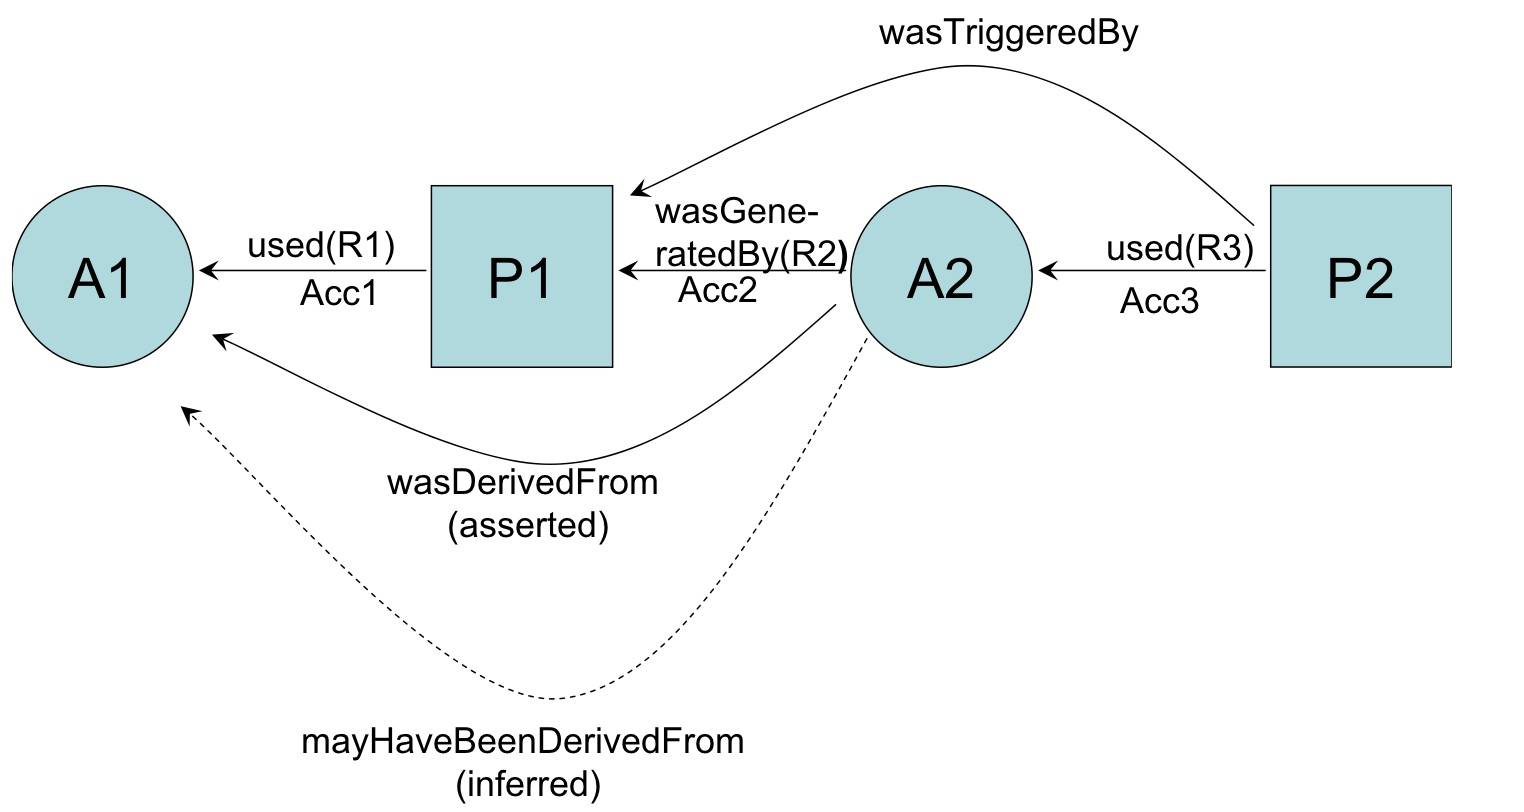
\includegraphics[width=\linewidth]{opm-example.jpg}
    \caption{Ejemplo de un proceso descrito utilizando \textit{OPM}.} Fuente:
    \textit{The Open Provenance Model}.
    \label{fig:opm-example}
\end{figure}

Una vez que hemos definido la procedencia de nuestros datos, podemos definir
otra información relacionada a su fuente tales cómo, autor, certeza de la
información y fuentes para así, a través de un proceso matemático
\cite{dividino2009provenance}, lograr calcular un valor a la confianza de los
datos disponibles. Este proceso, puede ser realizado a multiples fuentes,
sentencias y grafos, permitiendonos obtener un valor de confianza para
estructuras más complejas.

\subsubsection{Aplicaciones}
\label{sec:aplicaciones}

El paradigma basico para interactuar con datos es consultar y obtener una
respuesta: los usuarios construyen consultas y los sistemas entregan respuestas.
Por lo tanto, para que un sistema permita a los usuarios interactuar con sus
datos, necesita una interfaz que acepte consultas como entrada y muestre las
respuestas obtenidas desde el sistema de forma visual. En base a esto, muchas de
las actuales interfaces disponibles para interactuar con repositorios
\textit{RDF} o \textit{endpoints SPARQL} corresponden a interfaces interactivas
\textit{web}, como el \href{https://query.wikidata.org}{\textit{Wikidata Query
Service}} donde es posible realizar consultas y visualizar resultados de forma
interactiva (figuras \ref{fig:wikidata-ex-nobel} y
\ref{fig:wikidata-ex-nobel-result}).

\begin{figure}
    \centering
    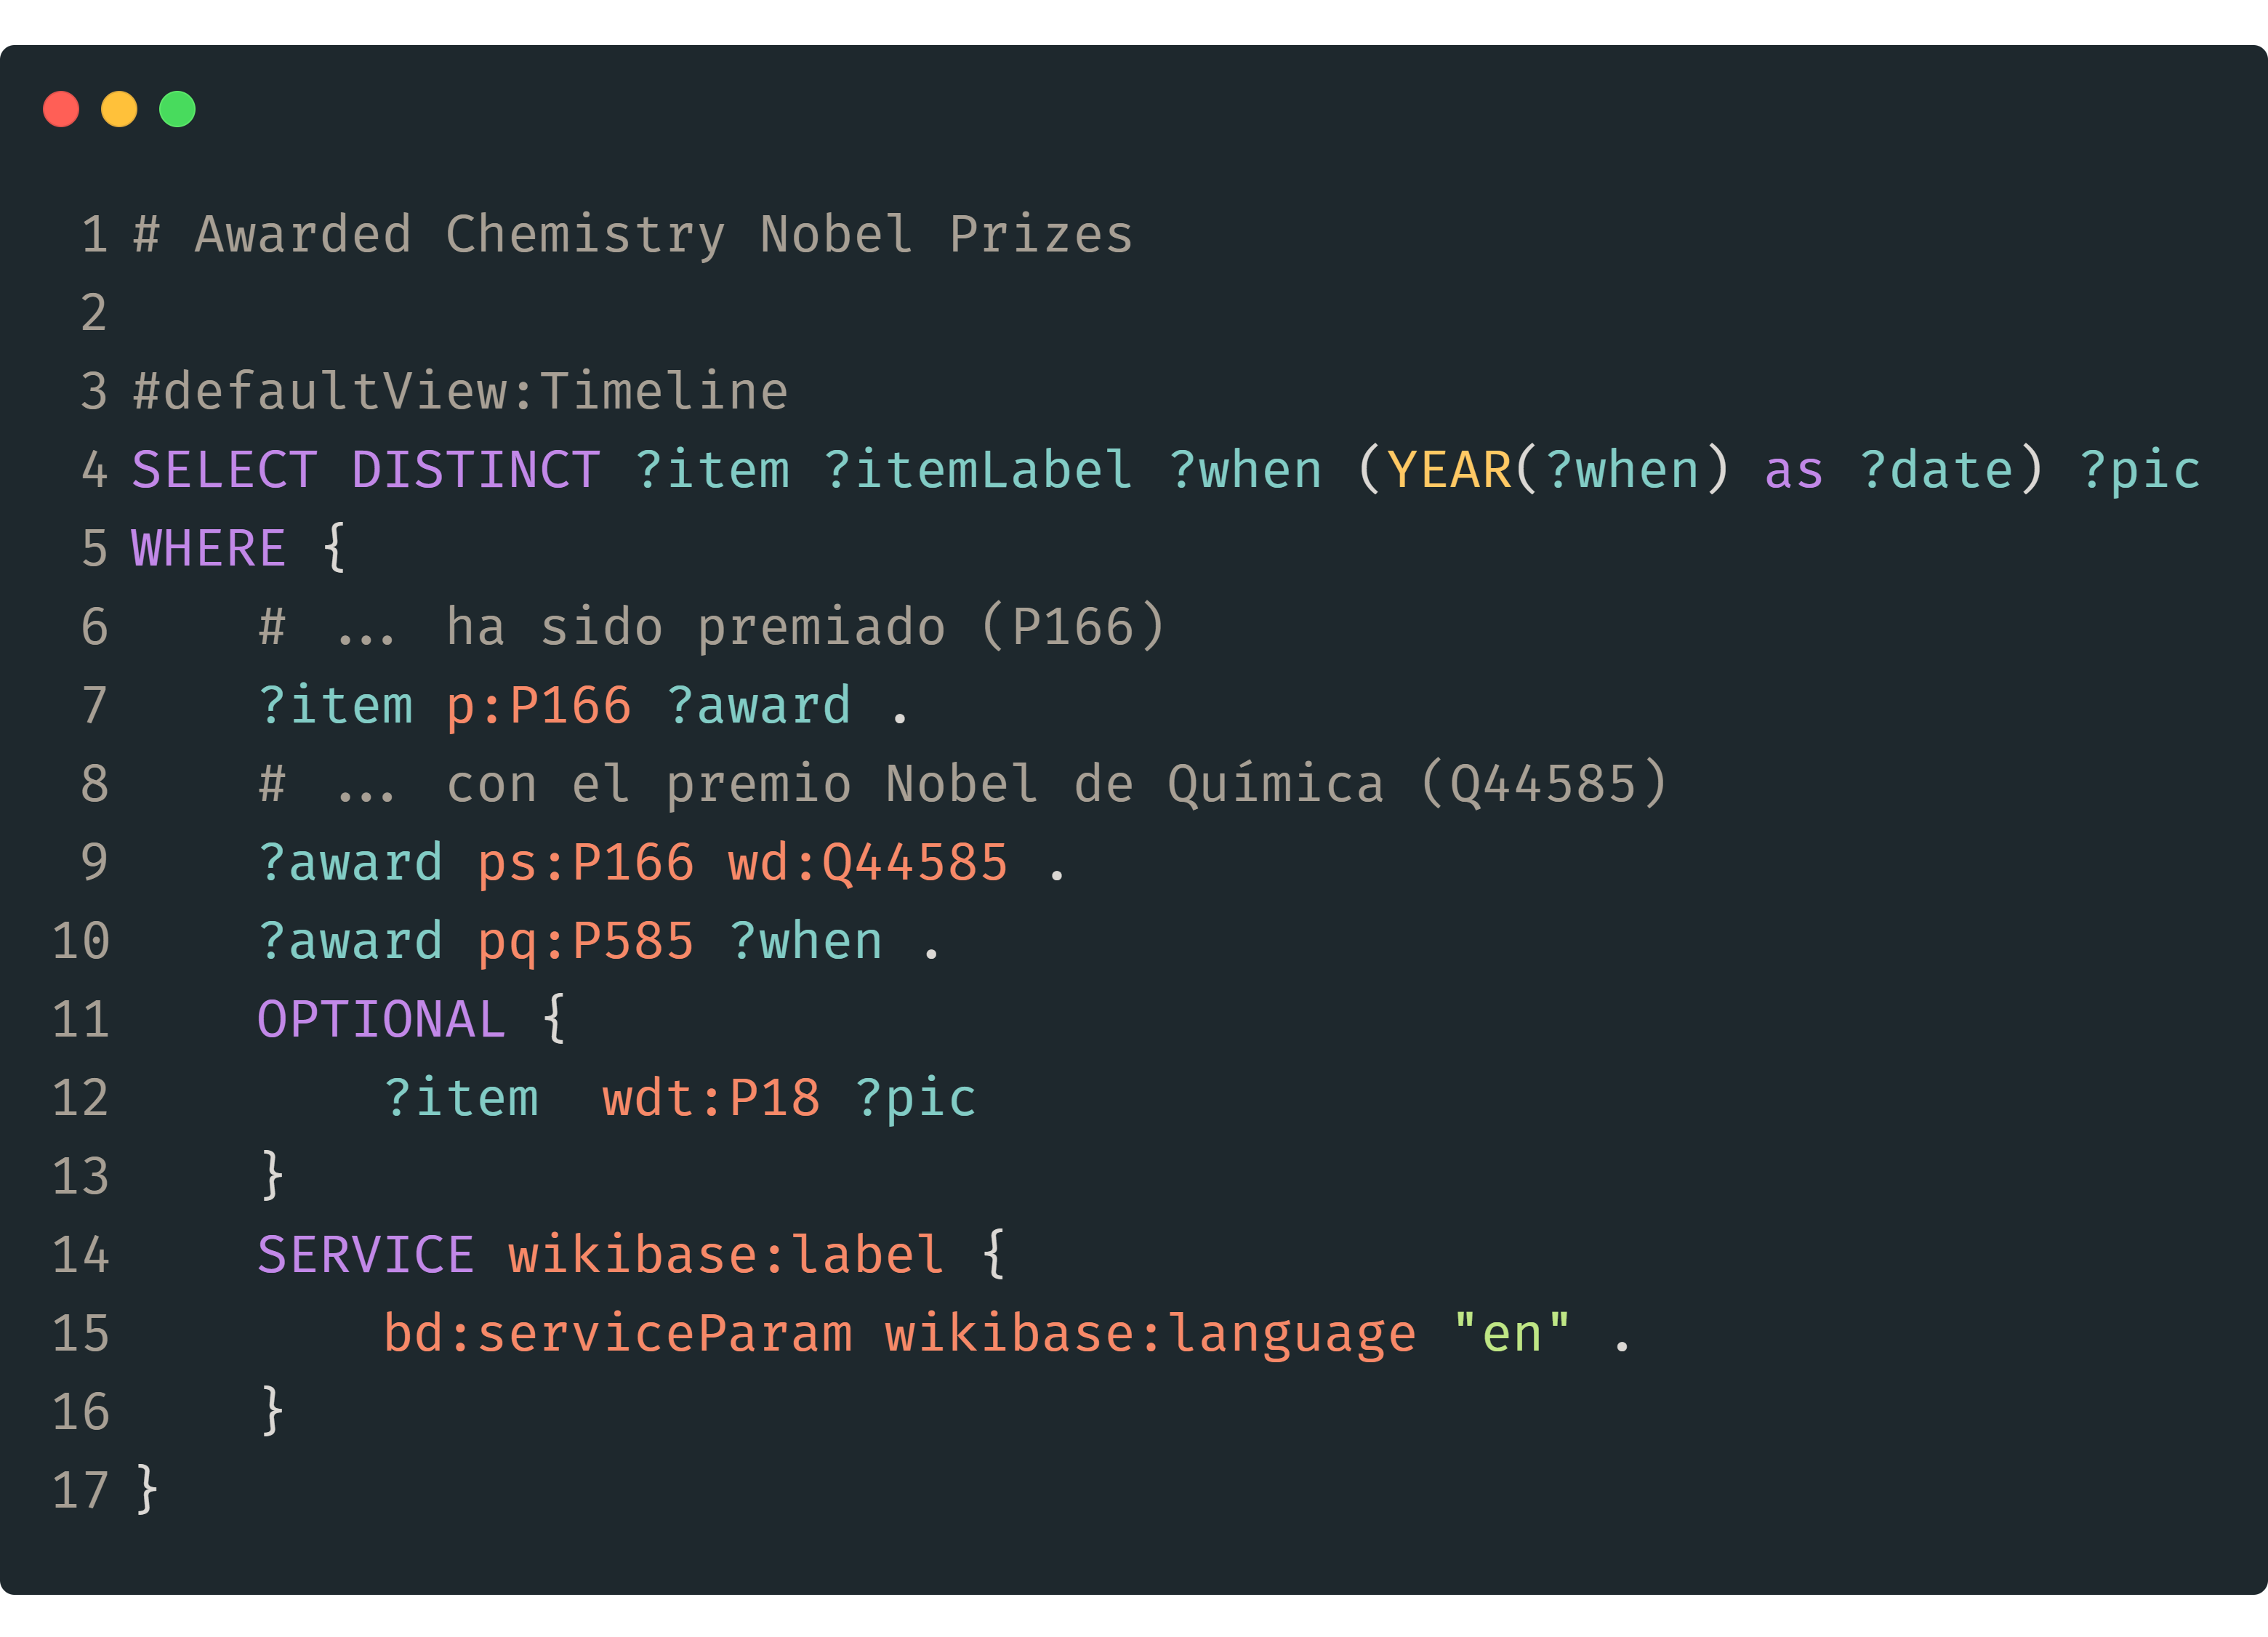
\includegraphics[width=\linewidth]{wikidata-ex-nobel.png}
    \caption{Consulta \textit{SPARQL} realizada en el \textit{Wikidata Query
    Service}.} Corresponde a obtener a aquellas personas que han sido premiadas
    con el Premio Nobel de Química. Fuente: Elaboración propia.
    \label{fig:wikidata-ex-nobel}
\end{figure}

\begin{figure}
    \centering
    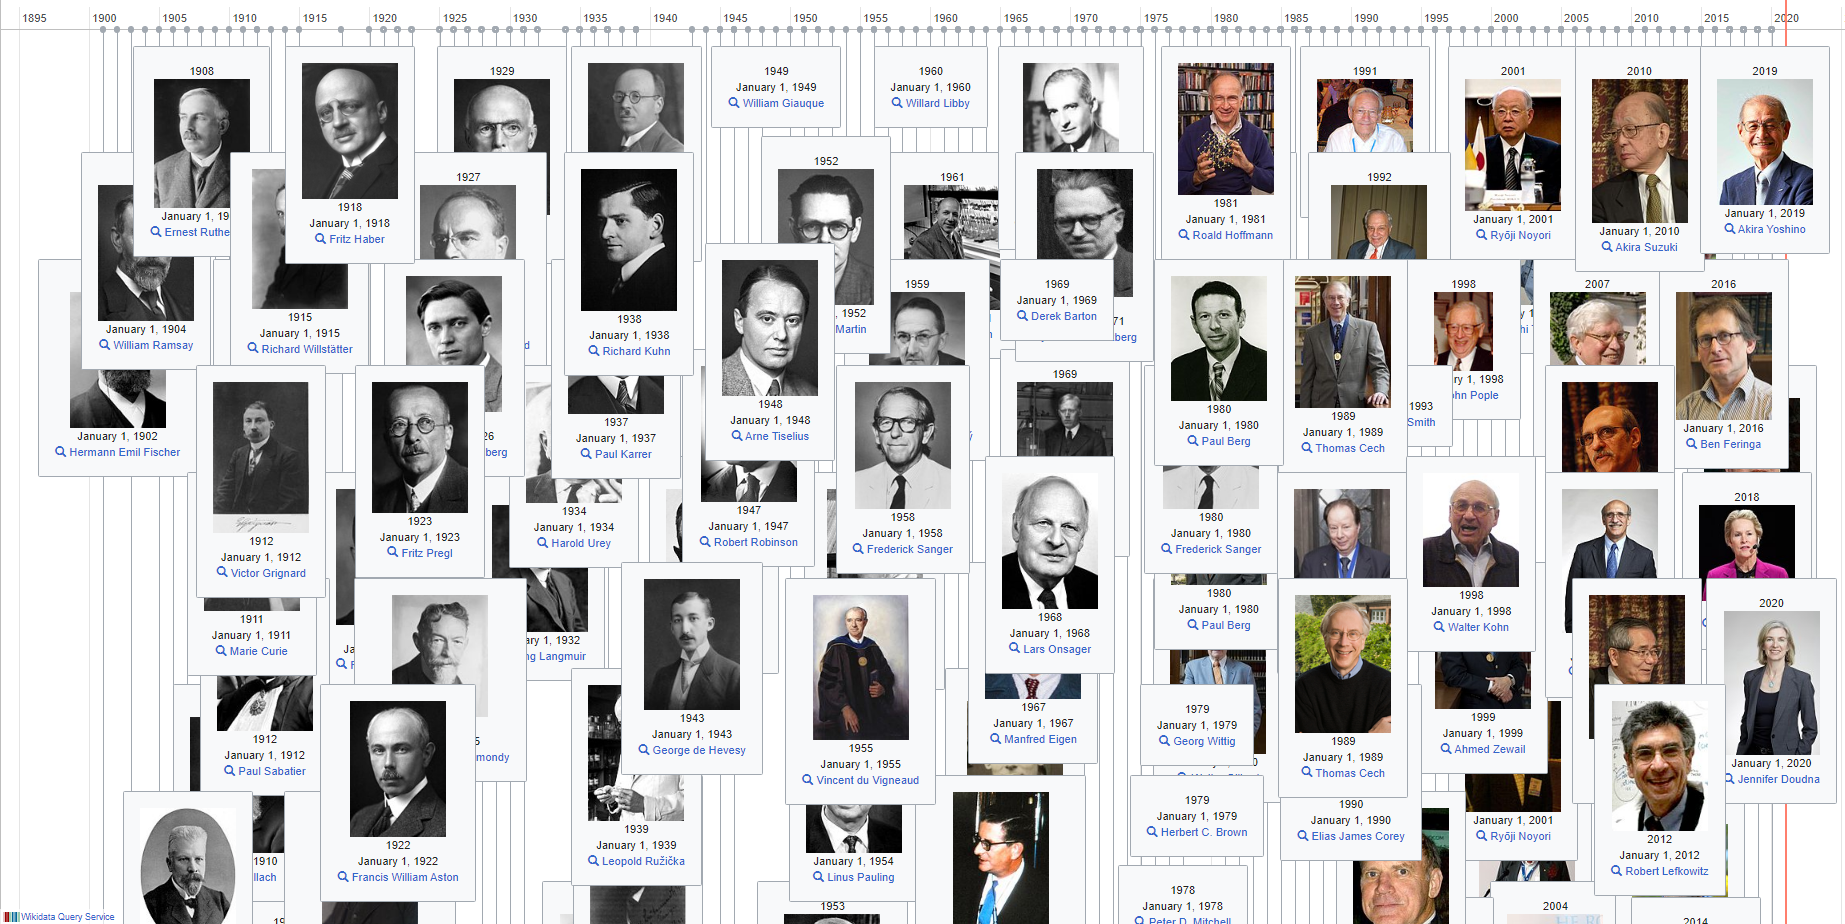
\includegraphics[width=\linewidth]{wikidata-ex-nobel-result.png}
    \caption{Visualización de una consulta \textit{SPARQL} en el
    \textit{Wikidata Query Service}.} Representa los resultados de obtener a
    aquellas personas que han sido premiadas con el Premio Nobel de Química
    Fuente: \textit{Wikidata Query Service}.
    \label{fig:wikidata-ex-nobel-result}
\end{figure}

La \textit{web} semántica genera nuevos desafios para el diseño y desarrollo de
interfaces que sean facil de utilizar para usuarios sin conocimientos tecnicos y
que permitan responder a preguntas del estilo ``¿Que tipo de musica se escucha
en las estaciones de radio de Alemania?'' o ``¿Que personas han participado en
la realización de peliculas sobre viajes en el tiempo?'' de forma rapida y
fluida.

En base a todas estas definiciones realizadas desde la sección
\ref{sec:refs-transporte-enlazados} hasta la sección \ref{sec:aplicaciones} es
que ahora podemos comprender que es la web semántica y resumirla como el
conjunto de herramientas, lenguajes, protocolos y estándares que permiten tanto
a humanos como a agentes inteligentes procesar toda la información disponible en
la \textit{web} a través de una base de datos global y distribuida.

\subsection{Generación de sugerencias}

El proceso de generación de sugerencias de entidades en base a consultas
\textit{SPARQL} parciales es la interfaz principal a nuestro sistema. Sin
embargo, para realizar este proceso, debemos ser capaces de conocer las
relaciones disponibles en nuestro conjunto de datos sin consultar directamente
al repositorio fuente. Para esto, crearemos un repositorio local que contendra
las entidades, identificadores, descripciones, relaciones y otras propiedades
necesarias para enviar las sugerencias a nuestros usuarios utilizando el
proyecto \textit{Apache Lucene} \cite{apache2012welcome}. Además, debido a la
gran cantidad de relaciones que pueden existir entre las entidades disponibles,
debemos generar un mecanismo que nos permita ordenar nuestros resultados por
relevancia. Utilizaremos el algoritmo \textit{PageRank} \cite{page1999pagerank}
para realizar este proceso.

\subsubsection{Indexación de documentos}
\label{sec:index-types}

Al buscar información sobre un documento de texto utilizando palabras claves,
estamos realizando una busqueda sobre el contenido de este texto. Para lograr
esto, necesitamos almacenar información sobre el contenido que estamos revisando
junto con la relación que indica como resultado, el identificador unico de la
fuente. Por ejemplo, cuando buscamos un libro a través del nombre de uno de sus
capitulos, las palabras claves son aquellas que se encuentran en el nombre del
capitulo y el identificador puede ser el nombre del libro. Este proceso de
busqueda se suele realizar a través de indices en bases de datos relacionales.

En el contexto de las bases de datos relacionales, los tipos de indicies más
conocidos son el indice delantero (\textit{forward index}) y en indice inverso
(\textit{inverse index}). Estrictamente hablando, no existe una diferencia
técnica en estos dos tipos de indices, puesto que la implementación es la misma
y es al momento de contextualizar el entorno en el que utilizaremos estos
indices donde se genera una diferencia. En el mundo de la busqueda de
documentos, un \textit{forward index} se construlle describiendo la relación
``El documento \texttt{id=doc1} contiene las palabras \texttt{el} y
\texttt{contenido}'', en cambio, un \textit{inverse index} nos presenta la
información de la forma ``La palabra \texttt{contenido} se encuentra en los
documentos \texttt{id=[doc1, doc2]}''. Una ilustración de este ejemplo se puede
observar en la figura \ref{fig:forward-backward-index}.

\begin{figure}
    \centering
    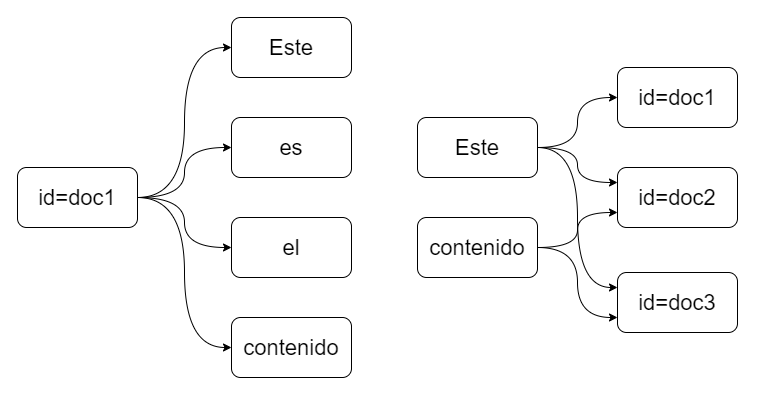
\includegraphics[width=\linewidth]{forward_backward_index.png}
    \caption{Ejemplos de un \textit{forward index} y un \textit{inverted
    index}.} A la izquierda \textit{forward index} y a la derecha
    \textit{inverted index}. Fuente: Elaboración propia.
    \label{fig:forward-backward-index}
\end{figure}

Nuestro repositorio local consiste en un \textit{inverse index}, en el cual, las
etiquetas, descripciones, propiedades y relaciones descritas en el grafo
\textit{RDF} apuntan al identeificador de la entidad descrita. De esta forma,
podemos buscar entidades utilizando sus propiedades de la misma forma en la que
buscamos un libro a través de su contenido.

Utilizaremos el proyecto \textit{Apache Lucene} \cite{apache2012welcome} para
lograr esta funcionalidad, puesto que, soporta estos y muchos tipos más de
indices para documentos de texto.

\subsubsection{\textit{Ranking} de resultados}

Una vez que hemos obtenido entidades para generar sugerencias, debemos entregar
a nuestro usuario las más relevantes para la consulta parcial que estamos
construyendo. Para esto, utilizaremos el algoritmo \textit{PageRank}
\cite{page1999pagerank}, el cual nos permite asignar un valor de importancia a
los resultados en base a la cantidad de conexiónes que cada elemento del grafo
\textit{RDF} tiene en relacion a sus propiedades y otras entidades.

\textit{PageRank} fue diseñado para agregar order e importancia a los resultados
de los primeros motores de busqueda en la \textit{web}. En el diseño del
algoritmo, los autores proponen que los sitios disponibles en la \textit{web}
están pueden ser modelados utilizando un grafo dirigido, en el cual, cada sitio
es un nodo del grafo y cada enlace hacia o desde estos sitios representa un arco
entre los nodos. Una vez que hemos construido nuestra representación, debemos
ejecutar nuestro algoritmo recursivo para asignar una alta importancia a
aquellos documentos que tienen muchos enlaces entrantes y pocos enlaces
salientes.

El proceso recursivo asigna un valor inicial al \textit{rank} todos los
documentos en la representación de forma tal que la suma de todos estos valores
es $1$. El siguiente paso es compartir el \textit{rank} de un documento entre
aquellos documentos a los que enlaza: un documento con alto \textit{rank}
entregará bastante puntaje a sus enlazados en comparación a un documento de bajo
\textit{rank} y con muchos enlaces salientes. Este proceso recursivo esta
asegurado para converger, por lo que despues de una cantidad de terminada de
iteraciones, el \textit{rank} de todos los documentos ha sido calculado.

El valor calculado por \textit{PageRank} es asignado los documentos almacenados
por \textit{Lucene} a través de un \textit{Document level
boosting}\footnote{\textit{Boosting:} Del inglés impulsar. En nuestro contexto,
se refiere a aumentar la importancia de una determinada variable a través de un
mecanismo externo.} el cual es aplicado a cada documento antes de ser ingresado
a nuestro \textit{reverse index} mencionado anteriormente.

\subsection{\textit{RDFExplorer}}

\textit{RDFExplorer} es...

\subsection{\textit{SPARQLforHumans}}

\textit{SPARQLforHumans} es...
